\section{Results}

% \begin{figure}[t]
% \center
% 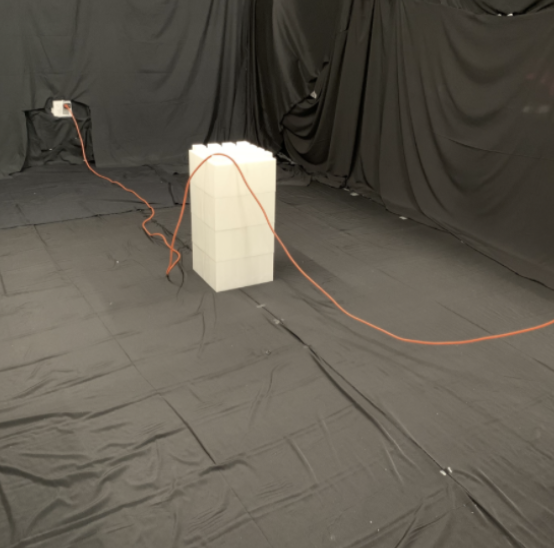
\includegraphics[width=34mm]{figures/failure.png}
% \caption{
% \small
% Failure case example. In this shown example, when the cable is too long (too slack), the motion that would have succeeded on a shorter cable fails to accomplish Task 1, and the resulting cable terminal configuration is not on the other side (right) of the obstacle, and instead the cable lands on the obstacle.
% }
% %\vspace*{-10pt}
% \label{fig:failure}
% \end{figure}
\begin{figure}[t]
    \vspace*{15pt}
    \centering
    % \begin{tabular}{c@{\hspace{1.5pt}}c@{\hspace{1.5pt}}}
    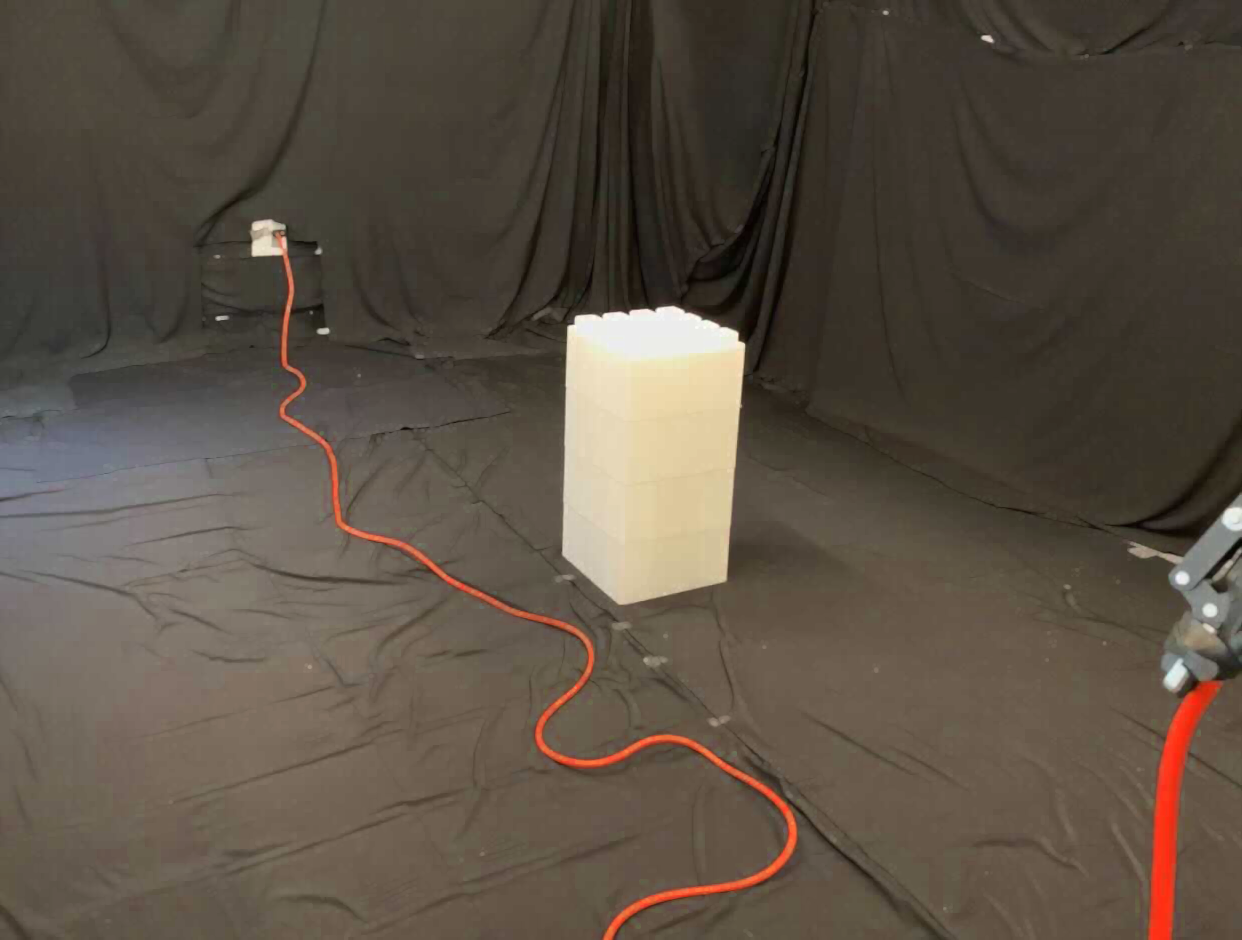
\includegraphics[width=120pt]{figures/failure_b4.png}\hfill
    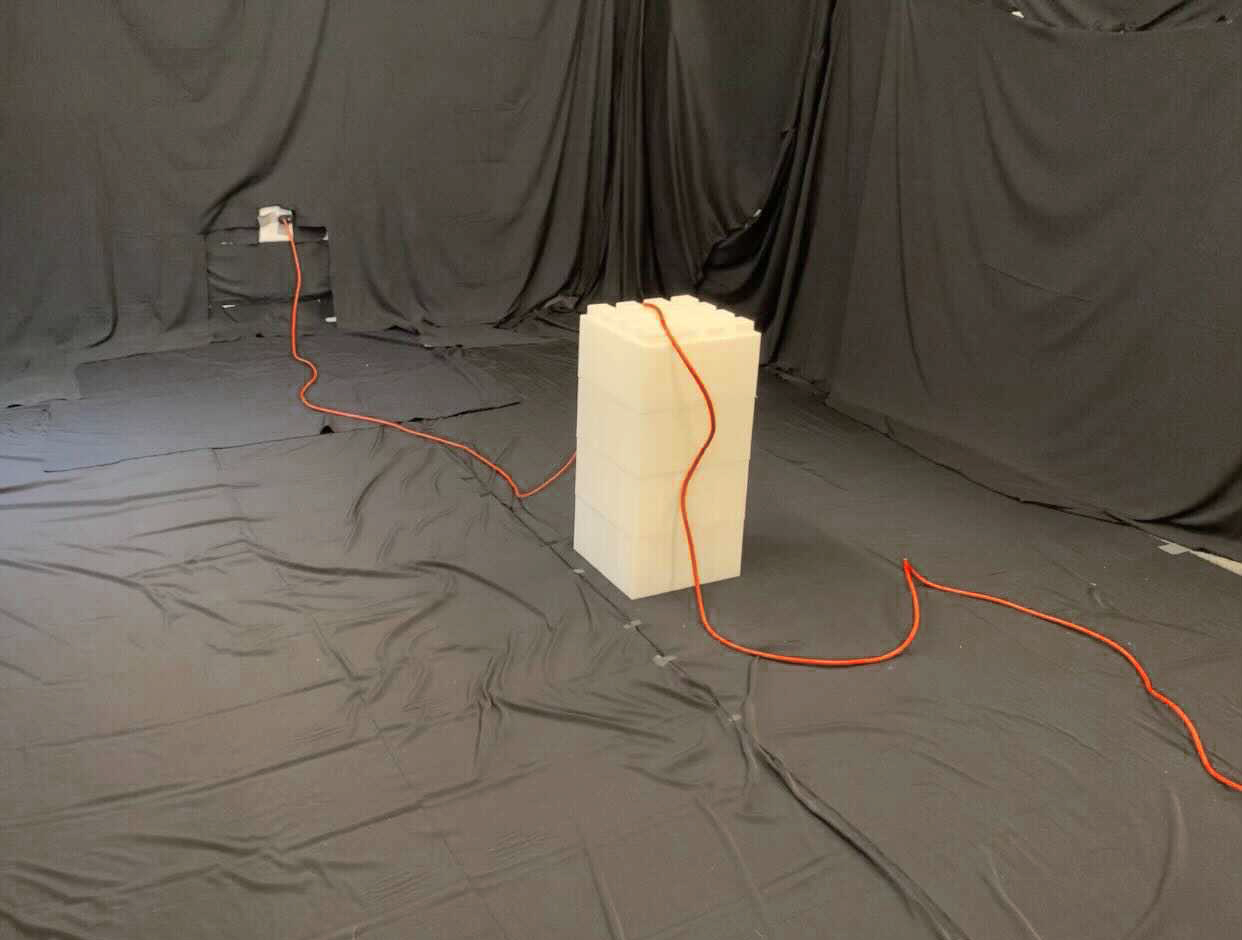
\includegraphics[width=120pt]{figures/failure_2.png}
    % \end{tabular}
    \caption{\textbf{Failure mode}. The 16-gauge 6.2~m orange cable is too long for the vaulting motion.  \textbf{Left:} before the motion there is too much slack. \textbf{Right:} the vaulting motion that works for shorter cables does not clear the obstacle.} %and the resulting cable terminal configuration is not on the other side (right) of the obstacle, and instead the cable lands on the obstacle.}
    
    \label{fig:failure}
\end{figure}

% The results suggest the learned policies can generalize to a variety of settings in terms of the objects' shapes and locations. 

We measure the correlation between simulated and real setups, benchmark the three dynamic cable tasks, and investigate generalization to different cables. %Across vaulting, knocking, and weaving, the learned apex procedure outperforms the baselines with fixed and varying apexes by 31.5\% and 16.5\%. 
%Since dynamic cable manipulating is best understood in action, We recommend viewing the supplementary videos on the project website.
The project website supplements these results with videos.

\subsection{Comparisons between Simulation and Reality}

To observe correlations between cable behavior in simulation and real, we evaluate vaulting on the same set of apex point and obstacle settings in both setups. Each trial consists of a random obstacle location from all 3 difficulty tiers and a different apex point. In simulation, we use a cube mesh of the same dimension as the plastic bricks obstacle in real, and a cable of the same length and mass as the 18 AWG orange cable. Table~\ref{table:sim_to_real} reports the frequency of success and failure cases across simulation and real. While the cable trajectory in simulation tends to match the trajectory of real for successes, 50\,\% of all failed cases in real succeed in simulation under the same setting. The discrepancies in cable behavior between simulation and real are most apparent for Tier 3 scenarios, where the height achieved by the cable at the opposite end from the robot differ in the two environments.  Because the cable properties cannot be perfectly tuned to match the physical properties in real, these experiments motivate the decision to use real experiments to collect data.
% 9 success cases and 6 failure cases from real are evaluated in the same conditions in simulation.

% \begin{tabular}{l|l|c|c|c}
% \multicolumn{2}{c}{}&\multicolumn{2}{c}{Real}&\\
% \cline{3-4}
% \multicolumn{2}{c|}{}&Successes&Failures&\multicolumn{1}{c}\\
% \cline{2-4}
% \multirow{2}{*}{Simulation}& Successes & $a$ & $b$\\
% \cline{2-4}
% & Failures & $c$ & $d$\\
% % \cline{2-4}
% % \multicolumn{1}{c}{} & \multicolumn{1}{c}{Total} & \multicolumn{1}{c}{$a+c$} & \multicolumn{    1}{c}{$b+d$} & \multicolumn{1}{c}{$N$}\\
% \end{tabular}

% \begin{table}
%     \vspace*{5pt}
% \centering
% \caption{Success rates of different vaulting apex points performed in simulation and real across 15 trials.}
% {    
% \begin{tabular}{cc|ccc}
% \multicolumn{2}{c}{}
%             &   \multicolumn{2}{c}{Real} \\
%     &   match   & differ &   Success &   Failure              \\ 
%     \cline{2-4}
% % \rotatebox[origin=c]{90}{Simulation}
%     Simulation
%     & Success   & 46.67\%&20\%\\
%     & Failure    & 13.33\%&20\%\\ 
%     \cline{2-4}
%     \end{tabular}
%     \vspace*{-10pt}
%  }
%  \label{table:sim_to_real}
% \end{table}
 
 \begin{table}
    \vspace*{4pt}
\centering
\caption{Number of successes and failures for vaulting in simulation and physical environments across 15 trials, evaluating a different apex point on a different obstacle position for each trial. Listed are the number of cases that succeed in both sim and real, fail in sim but succeed in real, succeed in sim but fail in real, and fail in both sim and real. The correlation between success rates in the two environments is surprisingly high.}
%\vspace{0.3cm}
 \begin{tabular}{ 
l c c}
% \multicolumn{4}{c}{Task 1 Results}\\
 \toprule
   & \#Success (Simulation) & \#Failure (Simulation) \\
  \midrule
  \#Success (Physical)&7&2\\
  \#Failure (Physical)&3&3\\
 \bottomrule
\end{tabular}
\vspace*{-5pt}

\label{table:sim_to_real}
\end{table}
\subsection{Results for Vaulting Task}
For vaulting, we perform 180 physical trials from manipulating the orange 5.5\,m 18-gauge power extension cable, with 60 trials for each of the 3 difficulty tiers; this process took 8 hours. In each tier, we shift the obstacle vertically within the bounds of the difficulty tier and horizontally within a range of 1.5\,m. We use plastic bricks to construct 6 combinations to build 6 objects of different sizes, and for each obstacle, we vary its location 10 times. Table~\ref{table:res_task1} shows results of the trained policy on vaulting evaluated with 20 trials per tier.

\begin{table}[t]
\vspace*{0pt}
\centering
\caption{Physical Vaulting Results: Number of successes of the learned policy for vaulting evaluated against two baseline methods across 20 trials per difficulty tier using the 18 AWG orange cable.}
%\vspace{0.3cm}
 \begin{tabular}{ 
l c c c}
% \multicolumn{4}{c}{Task 1 Results}\\
 \toprule
  Method & Tier 1 & Tier 2 & Tier 3\\
  \midrule
  Baseline with Fixed Apex&16&13&2\\
  Baseline with Varying Apex&19&14&7\\
  Learned Apex &\textbf{20}&\textbf{18}&\textbf{11}\\
 \bottomrule
\end{tabular}

\label{table:res_task1}
\end{table}

% For this task, we also evaluate the reversed-direction vaulting motion without training on the reversed-direction data. We reflect the input image and feed it into the network to plan a motion. It turns out we can accomplish reversed vaulting without actually training on reversed direction data. Intuitively, this is because since we are only regressing the midpoint (apex) of the motion, and we fix the starting and ending configurations of the robot, which are almost mirrored, the learned policy should be agnostic to the direction of vaulting. We achieve 100\% success in Tier 1, 80\% in Tier 2, and 50\% in Tier 3.
% Note that the result is slightly worse because the robot is not positioned perfectly in the center (slightly to the right), so the learned apex point is also conditioned on that center location.

\subsection{Results for Knocking Task}

For knocking, we perform 180 physical trials from manipulating the orange 5.5-m 18-gauge power extension cable, with 60 trials for each of 3 difficulty tiers; this process took 9 hours. In each difficulty tier, we use the plastic bricks as the base upon which we place the target object to be knocked, and we shift the plastic bricks base vertically within the bounds of the difficulty tier and horizontally within a range of 1.5\,m. We train the policy using four different target objects: a cylinder, a tennis ball, a cup, and a rectangular box. We use plastic bricks to construct 3 combinations to build 3 bases of different sizes. For each base, we vary its locations 5 times, and for each location of the base, we vary the target on top 4 times. 
%We also collect additional 30 trials using Hindsight Experience Replay (HER)~\cite{andrychowicz2017hindsight} in order to fully utilize the data. After we train with the 180 trials, we test the trained policy and collect all the failure cases where the cable lands on the Lego base but does not hit the object of interest. We take an image of the reset scene with the object placed at the location on the base where the cable landed and pretend that the object would have been hit successfully if it had been placed there, and the regression label remains the same as in the failure case. With these 30 additional trials, we finetune the trained network. 
Table~\ref{table:res_task2} shows the results for the knocking trained policy evaluated with 20 trials for each difficulty tier.% is shown in Table~\ref{table:res_task2}.
\begin{table}
\vspace*{4pt}
\centering
\caption{Physical Knocking Results: Number of successes of the learned policy for knocking evaluated against two baseline methods across 20 trials per difficulty tier using the 18 AWG orange cable.}
%\vspace{0.3cm}
 \begin{tabular}{ %p{2.8cm}||p{1cm}|p{1cm}|p{1cm}|p{1cm} | p{1cm}| p{1cm}| p{1cm}| p{1cm}|p{1cm}}
l c c c}
% \multicolumn{4}{c}{Task 2 Results}\\
 \toprule
  Method & Tier 1 & Tier 2 & Tier 3\\
  \midrule
  Baseline with Fixed Apex &12&6&4\\
  Baseline with Varying Apex &14&14&6\\

  Learned Apex&\textbf{15}&\textbf{14}&\textbf{10}\\
 \bottomrule
\end{tabular}
\label{table:res_task2}
\end{table}

\subsection{Results for Weaving Task}

We perform 100 physical trials from manipulating the orange 5.5-m 18-gauge power extension cable, which took 7.5 hours. We make the 3 obstacles identical in size. In our training data for this task, we vary the space between each object by 15 to 50\,cm and we shift the obstacles horizontally within a range of 1\,m.
%We evaluate weaving task by checking if the policy can produce two actions that manipulate a cable to be weaved between three objects. 
Table~\ref{table:res_task3} shows the result of the weaving trained policy evaluated with 20 trials. % is shown in Table~\ref{table:res_task3}.
% \begin{figure}
%     \vspace*{5pt}
%     \centering
%     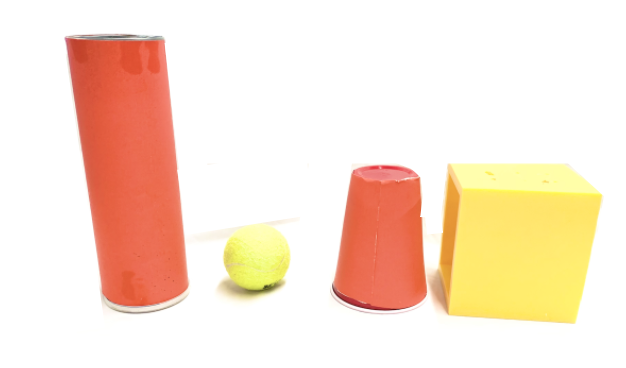
\includegraphics[width = 0.3\linewidth]{figures/targets.png}
%     \caption{Target objects used for training the knocking policy}
%     \label{fig:targets}
%     \vspace*{-10pt}
% \end{figure}

\subsection{Generalization to Different Cables}
%{\color{red} TODO: Add more details for each task and include number of trials per KG 10/29} 
While the policies for the three tasks are trained using the 18-gauge orange cable, we experiment with different types of cables. The results suggest that the policy trained on the 18-gauge orange cable can transfer well to other cables of similar lengths. We observe that the same reset action can bring these cables to nearly identical starting configurations in observation space, making the policy agnostic to cable type. We use the learned policy from the 18-gauge orange cable without retraining or finetuning to run the same experiments (same object sizes and locations for each task) for the 3 tasks with different cables and show results in Table~\ref{tab:cable_types}. 
%Using the 5.2-meter white 16-gauge cable, we achieve 80\% success rate for vaulting, 60\% success rate for knocking, and 60\% success rate for weaving. With the 5.5~m 22-gauge ethernet cable, we achieve 80\% success rate for vaulting, 50\% success rate for knocking, and 60\% success rate for weaving. With the 4.8~m 12-gauge jump rope, we achieve 80\% success rate for vaulting, 50\% success rate for knocking, and 40\% success rate for weaving.
\begin{table}
%\vspace*{-10pt}
\vspace*{0pt}
\centering
\caption{Physical Weaving Results: Number of successes of the learned policy for weaving evaluated against two baseline methods across 20 trials using the 18 AWG orange cable.}
%\vspace{0.3cm}
 \begin{tabular}{ %p{2.8cm}||p{1cm}|p{1cm}|p{1cm}|p{1cm} | p{1cm}| p{1cm}| p{1cm}| p{1cm}|p{1cm}}
l c c c}
% \multicolumn{4}{c}{Task 2 Results}\\
 \toprule
  Method & \#Success\\
  \midrule
  Baseline with Fixed Apex &3\\
  Baseline with Varying Apex &3\\

  Learned Apex&\textbf{12}\\
 \bottomrule
\vspace*{-10pt}
\end{tabular}
\label{table:res_task3}

\end{table}
\vspace*{-8pt}
\subsection{Limitations and Failure Modes}

While the framework can be robust to object locations and shapes, it has limitations. First, the policies are learned in a highly controlled environment. % where we constrain obstacles to a relatively small area.
Many failure cases in vaulting and knocking are from %outliers of 
placements outside the training area. For example, in Tier 3 vaulting, 7 of 9 failure cases are due to the horizontal shift of the obstacle exceeding the 1.5\,m bound. In weaving, the horizontal shift of the obstacles is bounded into a smaller 1.0\,m range.%so the trained weaving policy would not generalize to a variety of obstacles settings.
%
% Starting a paragraph with "Second," seems weird, unless we have a paragraph that starts with "First,"
Second, learned policies have difficulty generalizing to cables of different lengths and masses. We conjecture that with different lengths, the amount of slack in the cables should also be different, thus decreasing the repeatability of applying the same action. With the 6.2\,m cable, Tier 2 and 3 vaulting and knocking always fail in that the segment of the cable near the wall end can never be accelerated up due to the fact that the slack near the wall end cannot be eliminated by the resetting action.
%We hypothesize that this is the case because when the cable is too long, it would require more energy to be accelerated, and the energy generated from the action output by the policy trained on a shorter cable is lower than the expected energy, thus failing to manipulate the longer cable as desired. 
To show this failure mode with a longer cable, we run the policies for vaulting, knocking, and weaving trained with the 5.5-m 18-gauge cable on the 6.2-m 16-gauge cable, and we achieve 20\,\% success rate for vaulting, 10\,\% success rate for knocking, and 10\,\% success rate for weaving. Fig.~\ref{fig:failure} shows this failure case. Additionally, Table~\ref{tab:cable_types} suggests that cables that are too light are likely to yield lower success rates, which may be because they often travel slower during descent, limiting the distance the cable traverses. Finally, the data generation part in Alg.~\ref{alg:whip} is inefficient since when the obstacle size and location change, the algorithm needs to search for successful apex point again, so data generation in real is unable to record a wider variety of obstacle placements in an efficient manner.

% Lastly, our experiment environment is a highly controlled one and the obstacles and target objects we have used are fairly simple. More variations in the environment should be expected in real-life scenarios such as different obstacles and different target objects. To make the proposed system applicable in real life, we would need to collect more data from a variety of different obstacles and target objects or apply heavy domain randomization techniques to make the policy generalizable and we leave this to future work.

